%==============================================================================
% tento soubor pouzijte jako zaklad
% this file should be used as a base for the thesis
% Autoři / Authors: 2008 Michal Bidlo, 2016 Jaroslav Dytrych
% Kontakt pro dotazy a připomínky: dytrych@fit.vutbr.cz
% Contact for questions and comments: dytrych@fit.vutbr.cz
%==============================================================================
% kodovaní: UTF-8 (zmena prikazem iconv, recode nebo cstocs)
% encoding: UTF-8 (you can change it by command iconv, recode or cstocs)
%------------------------------------------------------------------------------
% zpracování / processing: make, make pdf, make clean
%==============================================================================
% Soubory, které je nutné upravit: / Files which have to be edited:
%   projekt-20-literatura-bibliography.bib - literatura / bibliography
%   projekt-01-kapitoly-chapters.tex - obsah práce / the thesis content
%   projekt-30-prilohy-appendices.tex - přílohy / appendices
%==============================================================================
\documentclass[]{fitthesis} % bez zadání - pro začátek práce, aby nebyl problém s překladem
%\documentclass[english]{fitthesis} % without assignment - for the work start to avoid compilation problem
%\documentclass[zadani]{fitthesis} % odevzdani do wisu - odkazy jsou barevné
%\documentclass[english,zadani]{fitthesis} % for submission to the IS FIT - links are color
%\documentclass[zadani,print]{fitthesis} % pro tisk - odkazy jsou černé
%\documentclass[zadani,cprint]{fitthesis} % pro barevný tisk - odkazy jsou černé, znak VUT barevný
%\documentclass[english,zadani,print]{fitthesis} % for the color print - links are black
%\documentclass[english,zadani,cprint]{fitthesis} % for the print - links are black, logo is color
% * Je-li prace psana v anglickem jazyce, je zapotrebi u tridy pouzit 
%   parametr english nasledovne:
%   If thesis is written in english, it is necessary to use 
%   parameter english as follows:
%      \documentclass[english]{fitthesis}
% * Je-li prace psana ve slovenskem jazyce, je zapotrebi u tridy pouzit 
%   parametr slovak nasledovne:
%      \documentclass[slovak]{fitthesis}

% Základní balíčky jsou dole v souboru šablony fitthesis.cls
% Basic packages are at the bottom of template file fitthesis.cls
%zde muzeme vlozit vlastni balicky / you can place own packages here

%---rm---------------
\renewcommand{\rmdefault}{lmr}%zavede Latin Modern Roman jako rm / set Latin Modern Roman as rm
%---sf---------------
\renewcommand{\sfdefault}{qhv}%zavede TeX Gyre Heros jako sf
%---tt------------
\renewcommand{\ttdefault}{lmtt}% zavede Latin Modern tt jako tt

% vypne funkci šablony, která automaticky nahrazuje uvozovky,
% aby nebyly prováděny nevhodné náhrady v popisech API apod.
% disables function of the template which replaces quotation marks
% to avoid unnecessary replacements in the API descriptions etc.
\csdoublequotesoff

% =======================================================================
% balíček "hyperref" vytváří klikací odkazy v pdf, pokud tedy použijeme pdflatex
% problém je, že balíček hyperref musí být uveden jako poslední, takže nemůže
% být v šabloně
% "hyperref" package create clickable links in pdf if you are using pdflatex.
% Problem is that this package have to be introduced as the last one so it 
% can not be placed in the template file.
\ifWis
\ifx\pdfoutput\undefined % nejedeme pod pdflatexem / we are not using pdflatex
\else
  \usepackage{color}
  \usepackage[unicode,colorlinks,hyperindex,plainpages=false,pdftex]{hyperref}
  \definecolor{links}{rgb}{0.4,0.5,0}
  \definecolor{anchors}{rgb}{1,0,0}
  \def\AnchorColor{anchors}
  \def\LinkColor{links}
  \def\pdfBorderAttrs{/Border [0 0 0] }  % bez okrajů kolem odkazů / without margins around links
  \pdfcompresslevel=9
\fi
\else % pro tisk budou odkazy, na které se dá klikat, černé / for the print clickable links will be black
\ifx\pdfoutput\undefined % nejedeme pod pdflatexem / we are not using pdflatex
\else
  \usepackage{color}
  \usepackage[unicode,colorlinks,hyperindex,plainpages=false,pdftex,urlcolor=black,linkcolor=black,citecolor=black]{hyperref}
  \definecolor{links}{rgb}{0,0,0}
  \definecolor{anchors}{rgb}{0,0,0}
  \def\AnchorColor{anchors}
  \def\LinkColor{links}
  \def\pdfBorderAttrs{/Border [0 0 0] } % bez okrajů kolem odkazů / without margins around links
  \pdfcompresslevel=9
\fi
\fi
% Řešení problému, kdy klikací odkazy na obrázky vedou za obrázek
% This solves the problems with links which leads after the picture
\usepackage[all]{hypcap}

% Informace o práci/projektu / Information about the thesis
%---------------------------------------------------------------------------
\projectinfo{
  %Prace / Thesis
  project=SP,            %typ prace BP/SP/DP/DR  / thesis type (SP = term project)
  year=2017,             %rok odevzdání / year of submission
  date=\today,           %datum odevzdani / submission date
  %Nazev prace / thesis title
  title.cs={Monitorování sítě - isamon},  %nazev prace v cestine ci slovenstine (dle zadani) / thesis title in czech language (according to assignment)
  title.en={Network monitoring - isamon}, %nazev prace v anglictine / thesis title in english
  %Autor / Author
  author={Vladimír Jeřábek},   %cele jmeno a prijmeni autora / full name and surname of the author
  author.name={Vladimír},   %jmeno autora (pro citaci) / author name (for reference) 
  author.surname={Jeřábek},   %prijmeni autora (pro citaci) / author surname (for reference) 
  %author.title.p=Bc., %titul pred jmenem (nepovinne) / title before the name (optional)
  %author.title.a=PhD, %titul za jmenem (nepovinne) / title after the name (optional)
  %Ustav / Department
  department=UIFS, % doplnte prislusnou zkratku dle ustavu na zadani: UPSY/UIFS/UITS/UPGM
  %                  fill in appropriate abbreviation of the department according to assignment: UPSY/UIFS/UITS/UPGM
  %Skolitel / supervisor
  supervisor=Jan Pluskal, %cele jmeno a prijmeni skolitele / full name and surname of the supervisor
  supervisor.name={Jan},   %jmeno skolitele (pro citaci) / supervisor name (for reference) 
  supervisor.surname={Pluskal},   %prijmeni skolitele (pro citaci) / supervisor surname (for reference) 
  supervisor.title.p=Ing.,   %titul pred jmenem (nepovinne) / title before the name (optional)
  %supervisor.title.a={},    %titul za jmenem (nepovinne) / title after the name (optional)
  %Klicova slova, abstrakty, prohlaseni a podekovani je mozne definovat 
  %bud pomoci nasledujicich parametru nebo pomoci vyhrazenych maker (viz dale)
  %Keywords, abstracts, declaration and acknowledgement can be defined by following 
  %parameters or using dedicated macros (see below)
  %===========================================================================
  %Klicova slova / keywords
  %keywords.cs={Klíčová slova v českém jazyce.}, %klicova slova v ceskem ci slovenskem jazyce
  %                                              keywords in czech or slovak language
  %keywords.en={Klíčová slova v anglickém jazyce.}, %klicova slova v anglickem jazyce / keywords in english
  %Abstract
  %abstract.cs={Výtah (abstrakt) práce v českém jazyce.}, % abstrakt v ceskem ci slovenskem jazyce
  %                                                         abstract in czech or slovak language
  %abstract.en={Výtah (abstrakt) práce v anglickém jazyce.}, % abstrakt v anglickem jazyce / abstract in english
  %Prohlaseni / Declaration
  %declaration={Prohlašuji, že jsem tuto bakalářskou práci vypracoval samostatně pod vedením pana ...},
  %Podekovani (nepovinne) / Acknowledgement (optional)
  %acknowledgment={Zde je možné uvést poděkování vedoucímu práce a těm, kteří poskytli odbornou pomoc.} % nepovinne
  %acknowledgment={Here it is possible to express thanks to the supervisor and to the people which provided professional help.} % optional
}

%Abstrakt (cesky, slovensky ci anglicky) / Abstract (in czech, slovak or english)
\abstract[cs]{Do tohoto odstavce bude zapsán výtah (abstrakt) práce v českém (slovenském) jazyce.}
\abstract[en]{Do tohoto odstavce bude zapsán výtah (abstrakt) práce v anglickém jazyce.}

%Klicova slova (cesky, slovensky ci anglicky) / Keywords (in czech, slovak or english)
\keywords[cs]{Sem budou zapsána jednotlivá klíčová slova v českém (slovenském) jazyce, oddělená čárkami.}
\keywords[en]{Sem budou zapsána jednotlivá klíčová slova v anglickém jazyce, oddělená čárkami.}

%Prohlaseni (u anglicky psane prace anglicky, u slovensky psane prace slovensky)
%Declaration (for thesis in english should be in english)
\declaration{Prohlašuji, že jsem tuto bakalářskou práci vypracoval samostatně pod vedením pana X...
Další informace mi poskytli...
Uvedl jsem všechny literární prameny a publikace, ze kterých jsem čerpal.}

% \declaration{Hereby I declare that this bachelor's thesis was prepared as an original author’s work under the supervision of Mr. X
% The supplementary information was provided by Mr. Y
% All the relevant information sources, which were used during preparation of this thesis, are properly cited and included in the list of references.}

%Podekovani (nepovinne, nejlepe v jazyce prace) / Acknowledgement (optional, ideally in the language of the thesis)
\acknowledgment{V této sekci je možno uvést poděkování vedoucímu práce a těm, kteří poskytli odbornou pomoc
(externí zadavatel, konzultant, apod.).}
%\acknowledgment{Here it is possible to express thanks to the supervisor and to the people which provided professional help
%(external submitter, consultant, etc.).}

% řeší první/poslední řádek odstavce na předchozí/následující stránce
% solves first/last row of the paragraph on the previous/next page
\clubpenalty=10000
\widowpenalty=10000

\begin{document}
  % Vysazeni titulnich stran / Typesetting of the title pages
  % ----------------------------------------------
  \maketitle
  % Obsah
  % ----------------------------------------------
  \setlength{\parskip}{0pt}

  {\hypersetup{hidelinks}\tableofcontents}
  
  % Seznam obrazku a tabulek (pokud prace obsahuje velke mnozstvi obrazku, tak se to hodi)
  % List of figures and list of tables (if the thesis contains a lot of pictures, it is good)
  \ifczech
    \renewcommand\listfigurename{Seznam obrázků}
  \fi
  \ifslovak
    \renewcommand\listfigurename{Zoznam obrázkov}
  \fi
  % \listoffigures
  
  \ifczech
    \renewcommand\listtablename{Seznam tabulek}
  \fi
  \ifslovak
    \renewcommand\listtablename{Zoznam tabuliek}
  \fi
  % \listoftables 

  \ifODSAZ
    \setlength{\parskip}{0.5\bigskipamount}
  \else
    \setlength{\parskip}{0pt}
  \fi

  % vynechani stranky v oboustrannem rezimu
  % Skip the page in the two-sided mode
  \iftwoside
    \cleardoublepage
  \fi

  % Text prace / Thesis text
  % ----------------------------------------------
  %=========================================================================
% (c) Michal Bidlo, Bohuslav Křena, 2008

\chapter{Úvod}
Nacházíme se v době, kdy už i naše pračky a ledičnky jsou připojeny k internetu a tím pádem s těmito zařízeními můžeme komunikovat vzdáleně. Avšak s přibývajicím počtem zařízení v internetu vyvstává otázka, jak moc jsou tyto  jednotlivé zařízení přístupné i pro nepovolané osoby.
\newline

S totuo problematikou sovisí také to, zda náhodou nemáme v konkrétní síti nějaké zařízení navíc, o kterém bychom nevěděli. 
\newline

Tento článek pojednává a programu \texttt{ISAMON}, který má sloužit pro monitorování sítě a pomoct při již zmiňovaných úskalích, které souvosí s rychle přibývajicmí počtem zařízení v síti.
\newline

V tomto článku však také nalezenete podrobnější informace o technice skenovaní, kterou tento program používá pro zjišťování například všech hostů, kteří jsou připojeni k internetu a nachází se v daném rozpětí sítě (více o tomto tématu v kapitole 2) a taktéž jaké techniky jsou použity pro skenování otevřených portů jak za pomocí protokolu TCP, tak i protokolu UDP (více v kapitole 3).
\newline

Dále je zde popsán způsob práce s tímto programem, a taktéž možné návratové kódy (více v kapitole 4).


\chapter{Hledání zařízení v síti}
Jednou ze základních služeb, která tento program nabízí uživatelům, tak je skenování zadané sítě pro nalezení všech aktivníh hostů, kteří jsou připojeni k internetu.
\newline

Všichni hosti jsou povini implemntovat \texttt{ICMP Echo server} funkci, dle \texttt{RFC 1122}. Tato funkce zajišťuje, že host korektně příjme \texttt{ICMP Echo request} a vygeneruje a pošle korespodnující \texttt{ICMP Echo replay}.\cite{RFC1122}

Jelikož né všechna zařízení respektují toto \texttt{RFC}, bylo nutné  implementovat dva rozdílné způsoby vyhledávání aktivních klientů. Jeden způsob je použit pro vyhledávání aktivních klientů v lokální síti a drůhý způsob pak při vyhledávání klientů ve vzdálené síti, kde vzdálená síť je definována, jako síť ve které není přítomné zařízení, na kterém běží program \texttt{ISAMON}.

\section{Způsob vyhledávání v lokální síti}
Jak již bylo popsáno výše, tak né každé zařízení respektuje implementaci \texttt{ICMP Echo server}, avšak vyhledávání v lokální síti je usnadněno existencí takzvaného \texttt{Adress Resolution Protocol (ARP)}, který zajišťuje překlad \texttt{IPv4} adresy na \texttt{MAC} adresu konkrétního zařízení. Jelikož bez implementace tohoto protokolu, by zařízení nebylo schopné poslat paket na jiné zařízení v síti, ba dokonce ani na směrovač, je tento protokol použit při skenování lokání sítě.
\newline



\subsection{Implementace skenování zařízení v lokání síti}
Skenování je založené na \texttt{ARP}. Na začátku skenování je vygenerován \textit{ethernetový rámec}, který je specifikován v \texttt{RFC 826}\cite{RFC826} a obsahuje konkrétní \texttt{IPv4} adresu hledaného zařízení v síti. Pro odeslání \texttt{ARP} rámce bylo zapotřebí použít takzvaný \textit{RAW socket}. 

Pokud zařízení s konkrétní \texttt{IPv4} adresu existuje v lokální síti, tak je vygenerována patřičná odpověď a program \texttt{ISAMON} tuto odpověď zachytí a přidá \texttt{IPv4} adresu tohoto zařízení do instance třídy \texttt{IsamonLiveVect}, což je speciální vektor, který udržuje informace o aktivních zařízeních ve skenované síti.

Pokud však zařízení v síti neexistuje, program \texttt{ISAMON} žádnou odpověď nezachytí a po vypršení časovače přestane čekat na odpověď a považuje zařízení za neaktivní, tudíž toto zařízení není přidáno do instance třídy \texttt{IsamonLiveVect}, a nebude na něm prováděno případné další skenování.
\newline

Pozn: Při pokoušení se oskenovat sám sebe, není poslán ARP dotaz, protože by byl bezdůvodný (\textit{tzv: Gratuitous}), přičemž by se nevygenerovala patřičná odpoveď a tím pádem by se naše zařízení tvářilo jako by bylo neaktivní. V tomto případě se přistupuje k vlastnímu zařízení jako kdyby toto zařízení bylo ve vzdálení síti, avšak musí se naslouchat na takzvaném \textit{loopback} zařízení.

\section{Způsob vyhledávání ve vzdálené síti}
Zde se nám nabízí jen několik málo různých přístupů k prohledávání vzdálené sítě a jedním z nich je použití protokolu \texttt{Internet Control Message Protocol (ICMP)}, avšak počítá se s tím, že v síti se některé pakety mohou ztratit (tzn. nedorazí k cíli), popřípadě mohou být zahozeny (vypršení TTL), takže tento způsob není vždy dokonalý.

\subsection{Implementace skenování zařízení ve vzdálené síti}
Při začátku skenování tohoto vzdáleného zařízení se na začátku vytvoří paket, dle popisu v \texttt{RFC 792}\cite{RFC792}, tomuto paketu se přenastaví TTL na co nejvyšší hodnotu (konkrétně \textit{255}), aby se předešlo zahazování paketů, a daný sestavený paket se pomocí specifického rozhraní pošle do sítě. 

Pokud zařízení s konkrétní \texttt{IPv4} adresu existuje a taktéž na tomto zařízení je korektně implementován \texttt{ICMP Echo server}, tak  tak vygeneruje patřičnou odpověď (jedná se \textit{ICMP Echo replay}) a tato odpověď je zachycena programem \texttt{ISAMON} a poté zpracována. Výsledkem zpracování je přidání adresy tohoto aktivního zařízení do instance třídy \texttt{IsamonLiveVect}.

Pokud však zařízení v síti neexistuje, nebo na tomto zařízení není korektně implementován \texttt{ICMP Echo server}, program \texttt{ISAMON} žádnou odpověď nezachytí a po vypršení časovače přestane čekat na odpověď a považuje zařízení za neaktivní, tudíž toto zařízení není přidáno do instance třídy \texttt{IsamonLiveVect}, a nebude na něm prováděno případné další skenování.



\chapter{Skenování portů u aktivních zařízení}
Jednou z dalších důležitých služeb, které jsou implementovány v programu \texttt{ISAMON} je možnost skenovat otevřené porty na jednotlivých aktivních zařízeních za pomoci rozdílných protokolů, jako je UDP \cite{RFC768} nebo TCP \cite{RFC793}.

Jelikož přistupování k těmto protokolům je značně odlišné, jsou jednotlivé techniky skenování popsány ve zvláštních kapitolách.

\section{Skenování TCP portů}
Protokol TCP zajišuje \textit{spojení} dvou zařízení, která se nachází v internetové síti a tento protokol garantuje spolehlivé doručování zpráv oběma směry. Na začátku spojení dvou zařízení pomocí tohoto protokolu je vždy takzvaný \textit{TCP handshake} (viz obrázek), který zajišťuje, že o sobě dané dvě zařízení ví a jsou připraveny na vzájemnou komunikaci. 
\newline

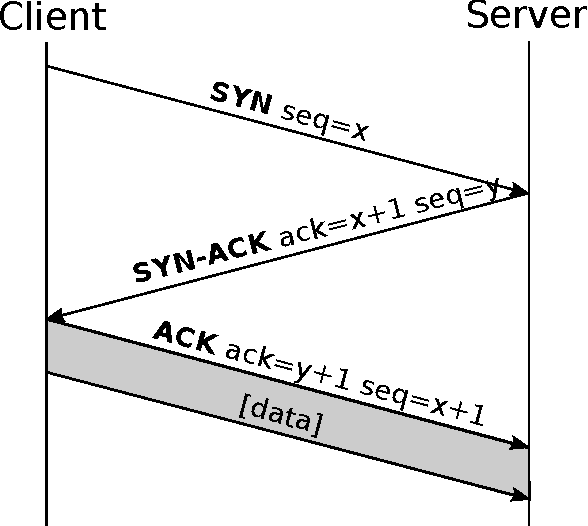
\includegraphics{obrazky-figures/Tcp-handshake.pdf}

Tohoto způsobu je využito i při scenování TCP portů. Na začátku program \texttt{ISAMON} zašle TCP paket s příznakem \textit{SYN} na konkrétní port u aktivního skenovaného hosta a očekává, že příjde paket s nastavenými příznaky buď \textit{SYN-ACK} (v tomto případě je port otevřený), a nebo příjde paket s nastaveným příznakem \textit{RST} (v tomto případě jde o zavřený port).

\subsection{Implemetace skenování TCP portů}
 Na začátku skenování pomocí TCP je otevřen \textit{TCP socket}, kterým zajistíme, že odeslaný paket bude mít formát a strukturu pospanou v \texttt{RFC 793} \cite{RFC793}. 
 
 Dále je nastaveno internetové rozhraní, které bude sloužit pro komunikaci mezi zařízeními. Jelikož požadujeme, aby skenování bylo co nejrychlejší, tak je použit neblokujicí \textit{connect}, který nám dovoluje nečekat na potvrzovací pakety a popřípadě zasílat na jiný port či jiného aktivního hosta další požadavky. 
 
 Příchozí pakety jsou odchytáváný za pomocí aplikačního rzhraní zvaného \textit{libpcap}, které dokáže zpracovávat odchycené pakety. Pokud je tedy odchycen paket, který má nastavený příznak \textit{SYN-ACK}, pak je tento port přidán jako otevřený ke konkrétnímu aktivnímu hostu.

\section{Skenování UDP portů}
Protokol UDP je, oproti TCP protokolu, \textit{nespojovaný} a taktéž nezaručuje doručení paketů. V UDP protokolu neexistuje ani nic jako v TCP \textit{TCP handshake}, který by nás informoval o povedení spojení, či ne. Jediné však co je generované a podel čeho lze usoudit, zda daný UDP port je otevřen, či zavřen, tak je informace ohledně nedostupnosti portu, kde tato informace je přenáčena protokolem \texttt{ICMP} a nazývá se obecně \textit{Port Unreachable}\cite{RFC1122}. Jediný možný způsob tedy je, že jsou odeslána data na dané aktivní zařízení a konkrétní UDP port a čeká se jestli se navrátí \textit{ICMP Port unreachable}, a nebo se nevratí nic.

\subsection{Implemetace skenování UDP portů}
Na začátku skenování pomocí UDP je otevřen \textit{UDP socket}.

Dále je nastaveno internetové rozhraní, které bude sloužit pro komunikaci mezi zařízeními. Poté se již odešle prázdná zpráva s délkou 0 na daný UDP port daného aktivního klienta.

Příchozí pakety jsou odchytáváný za pomocí aplikačního rzhraní zvaného \textit{libpcap}, které dokáže zpracovávat odchycené pakety. Pokud je odchycen \textit{ICMP} packet, jehož \textit{type} a \textit{code} odpovídá \textit{Port unreachable}, pak je zřejmé, že tento port je zavřen.

Avšak pokud do vypršení časovačče nedostaneme odpověď, pak si jen můžeme domyslet, že daný port je otevřen.
\newline

Pozn: Skenování UDP portů je velmi nepřesné a taktž velmi zdlouhavé. V realém nasazení né každý host má naimplementovaný \textit{ICMP Destination port unreachable}, protože tato funkcionalita je pouze doporučená a né přikázaná. Dalším úskalím, které se oběvuje při skenovní UDP portů, tak je omezní počtu poslaných \textit{ICMP} zpráv za jednotku času.



\chapter{Použití programu \texttt{ISAMON}}
Jak lze spouštěť:
\newline
\texttt{isamon [-h] [-i <interfc>] [-t] [-u] [-p <port>] [-w <ms>] -n <net\_addr/mask> }

\texttt{-h -{}-help} $\Rightarrow$ zobrazení nápovědy

\texttt{-i -{}-interface <interface>} $\Rightarrow$ rozhraní na kterém bude nástroj scanovat

\texttt{-n -{}-network <net\_address/mask>} $\Rightarrow$ ip adresa síťe s maskou definující rozsah pro scanování 

\texttt{-t -{}-tcp} $\Rightarrow$ použije TCP 

\texttt{-u -{}-udp} $\Rightarrow$ použije UDP 

\texttt{-p -{}-port <port>} $\Rightarrow$ specifikace scanovaného portu, pokud není zadaný, scanujte celý rozsah

\texttt{-w -{}-wait <ms>} $\Rightarrow$ jak dlouho se bude čekat na odpověď (výchozí nastavení jsou 2 sekundy)
\newline

\section{Příklady použití}
Pár příkladů:

\texttt{\$ isamon -h } $\Rightarrow$ vypíše se nápověda
\newline

\texttt{\$ isamon -i eth0 -n 192.168.1.0/24} 

$\Rightarrow$ provede se scanování sítě a zobrazí se aktivní klienti za použití rozhraní eth0
\newline

\texttt{\$ isamon -n 192.168.1.0/30}

$\Rightarrow$ provede se scanování sítě a zobrazí se aktivní klienti za použití všech rozhraní 
\newline

\texttt{\$ isamon -n 192.168.1.0/28 -t -p 22}

$\Rightarrow$ provede se scanování sítě a zobrazí se aktivní klienti s otevřeným TCP portem 22 za použití všech rozhraní 
\newline

\texttt{\$ isamon -n 192.168.1.0/30 -t -u -w 5}

$\Rightarrow$ provede se scanování sítě a zobrazí se aktivní klienti a všechny otevřené TCP a UDP porty za použití všech rozhraní, pokud klient neodpoví do 5ms, daný port je povaován za uzavřený

\section{Návratové kódy}
Program \texttt{ISAMON} může skončit s těmito návratovými kódy:

	\texttt{0} : Všechno probělo v pořádku
	
	\texttt{1} : CHYBA - v parsování argumentů
	
	\texttt{2} : CHYBA - v nastavení adresy sítě či masky
	\newline
	
	\texttt{5} : CHYBA - způsobená při získávání informací o rozhraních
	
	\texttt{6} : CHYBA - ve vytváření nebo odesílání ICMP packetu
	
	\texttt{7} : CHYBA - při vytváření TCP soketu 
	
	\texttt{8} : CHYBA - při vytváření či odesílání UDP packetu
	\newline
	
	\texttt{10} : CHYBA - při odchytávání packétu (pcap chyba)
	
	




%=========================================================================
 % viz. obsah.tex / see obsah.tex

  % Pouzita literatura / Bibliography
  % ----------------------------------------------
\ifslovak
  \makeatletter
  \def\@openbib@code{\addcontentsline{toc}{chapter}{Literatúra}}
  \makeatother
  \bibliographystyle{bib-styles/czechiso}
\else
  \ifczech
    \makeatletter
    \def\@openbib@code{\addcontentsline{toc}{chapter}{Literatura}}
    \makeatother
    \bibliographystyle{bib-styles/czechiso}
  \else 
    \makeatletter
    \def\@openbib@code{\addcontentsline{toc}{chapter}{Bibliography}}
    \makeatother
    \bibliographystyle{bib-styles/englishiso}
  %  \bibliographystyle{alpha}
  \fi
\fi
  \begin{flushleft}
  \bibliography{projekt-20-literatura-bibliography}
  \end{flushleft}

  % vynechani stranky v oboustrannem rezimu
  % Skip the page in the two-sided mode
  \iftwoside
    \cleardoublepage
  \fi

  % Prilohy / Appendices
  % ---------------------------------------------
  \appendix
\ifczech
  \renewcommand{\appendixpagename}{Přílohy}
  \renewcommand{\appendixtocname}{Přílohy}
  \renewcommand{\appendixname}{Příloha}
\fi
\ifslovak
  \renewcommand{\appendixpagename}{Prílohy}
  \renewcommand{\appendixtocname}{Prílohy}
  \renewcommand{\appendixname}{Príloha}
\fi
%  \appendixpage

% vynechani stranky v oboustrannem rezimu
% Skip the page in the two-sided mode
%\iftwoside
%  \cleardoublepage
%\fi
  
\ifslovak
%  \section*{Zoznam príloh}
%  \addcontentsline{toc}{section}{Zoznam príloh}
\else
  \ifczech
%    \section*{Seznam příloh}
%    \addcontentsline{toc}{section}{Seznam příloh}
  \else
%    \section*{List of Appendices}
%    \addcontentsline{toc}{section}{List of Appendices}
  \fi
\fi
  \startcontents[chapters]
  \setlength{\parskip}{0pt}
  % seznam příloh / list of appendices
  % \printcontents[chapters]{l}{0}{\setcounter{tocdepth}{2}}
  
  \ifODSAZ
    \setlength{\parskip}{0.5\bigskipamount}
  \else
    \setlength{\parskip}{0pt}
  \fi
  
  % vynechani stranky v oboustrannem rezimu
  \iftwoside
    \cleardoublepage
  \fi
  %% Tento soubor nahraďte vlastním souborem s přílohami (nadpisy níže jsou pouze pro příklad)
% This file should be replaced with your file with an appendices (headings below are examples only)

% Umístění obsahu paměťového média do příloh je vhodné konzultovat s vedoucím
% Placing of table of contents of the memory media here should be consulted with a supervisor
%\chapter{Obsah přiloženého paměťového média}

%\chapter{Manuál}

%\chapter{Konfigurační soubor} % Configuration file

%\chapter{RelaxNG Schéma konfiguračního souboru} % Scheme of RelaxNG configuration file

%\chapter{Plakát} % poster

\chapter{Jak pracovat s touto šablonou}
\label{jak}

V této kapitole je uveden popis jednotlivých částí šablony, po kterém následuje stručný návod, jak s touto šablonou pracovat. 

Jedná se o přechodnou verzi šablony. Nová verze bude zveřejněna do~konce roku 2017 a~bude navíc obsahovat nové pokyny ke správnému využití šablony, závazné pokyny k~vypracování bakalářských a diplomových prací (rekapitulace pokynů, které jsou dostupné na~webu) a nezávazná doporučení od vybraných vedoucích, která již teď najdete na~webu (viz odkazy v souboru s literaturou). Jediné soubory, které se v nové verzi změní, budou \texttt{projekt-01-kapitoly-chapters.tex} a \texttt{projekt-30-prilohy-appendices.tex}, jejichž obsah každý student vymaže a nahradí vlastním. Šablonu lze tedy bez problémů využít i~v~současné verzi.

\section*{Popis částí šablony}

Po rozbalení šablony naleznete následující soubory a adresáře:
\begin{DESCRIPTION}
  \item [bib-styles] Styly literatury (viz níže). 
  \item [obrazky-figures] Adresář pro Vaše obrázky. Nyní obsahuje placeholder.pdf (tzv. TODO obrázek, který lze použít jako pomůcku při tvorbě technické zprávy), který se s prací neodevzdává. Název adresáře je vhodné zkrátit, aby byl jen ve zvoleném jazyce.
  \item [template-fig] Obrázky šablony (znak VUT).
  \item [fitthesis.cls] Šablona (definice vzhledu).
  \item [Makefile] Makefile pro překlad, počítání normostran, sbalení apod. (viz níže).
  \item [projekt-01-kapitoly-chapters.tex] Soubor pro Váš text (obsah nahraďte).
  \item [projekt-20-literatura-bibliography.bib] Seznam literatury (viz níže).
  \item [projekt-30-prilohy-appendices.tex] Soubor pro přílohy (obsah nahraďte).
  \item [projekt.tex] Hlavní soubor práce -- definice formálních částí.
\end{DESCRIPTION}

Výchozí styl literatury (czechiso) je od Ing. Martínka, přičemž anglická verze (englishiso) je jeho překladem s drobnými modifikacemi. Oproti normě jsou v něm určité odlišnosti, ale na FIT je dlouhodobě akceptován. Alternativně můžete využít styl od Ing. Radima Loskota nebo od Ing. Radka Pyšného\footnote{BP Ing. Radka Pyšného \url{http://www.fit.vutbr.cz/study/DP/BP.php?id=7848}}. Alternativní styly obsahují určitá vylepšení, ale zatím nebyly řádně otestovány větším množstvím uživatelů. Lze je považovat za beta verze pro zájemce, kteří svoji práci chtějí mít dokonalou do detailů a neváhají si nastudovat detaily správného formátování citací, aby si mohli ověřit, že je vysázený výsledek v pořádku.

Makefile kromě překladu do PDF nabízí i další funkce:
\begin{itemize}
  \item přejmenování souborů (viz níže),
  \item počítání normostran,
  \item spuštění vlny pro doplnění nezlomitelných mezer,
  \item sbalení výsledku pro odeslání vedoucímu ke kontrole (zkontrolujte, zda sbalí všechny Vámi přidané soubory, a případně doplňte).
\end{itemize}

Nezapomeňte, že vlna neřeší všechny nezlomitelné mezery. Vždy je třeba manuální kontrola, zda na konci řádku nezůstalo něco nevhodného -- viz Internetová jazyková příručka\footnote{Internetová jazyková příručka \url{http://prirucka.ujc.cas.cz/?id=880}}.

\paragraph {Pozor na číslování stránek!} Pokud má obsah 2 strany a na 2. jsou jen \uv{Přílohy} a~\uv{Seznam příloh} (ale žádná příloha tam není), z nějakého důvodu se posune číslování stránek o 1 (obsah \uv{nesedí}). Stejný efekt má, když je na 2. či 3. stránce obsahu jen \uv{Literatura} a~je možné, že tohoto problému lze dosáhnout i jinak. Řešení je několik (od~úpravy obsahu, přes nastavení počítadla až po sofistikovanější metody). \textbf{Před odevzdáním proto vždy překontrolujte číslování stran!}


\section*{Doporučený postup práce se šablonou}

\begin{enumerate}
  \item \textbf{Zkontrolujte, zda máte aktuální verzi šablony.} Máte-li šablonu z předchozího roku, na stránkách fakulty již může být novější verze šablony s~aktualizovanými informacemi, opravenými chybami apod.
  \item \textbf{Zvolte si jazyk}, ve kterém budete psát svoji technickou zprávu (česky, slovensky nebo anglicky) a svoji volbu konzultujte s vedoucím práce (nebyla-li dohodnuta předem). Pokud Vámi zvoleným jazykem technické zprávy není čeština, nastavte příslušný parametr šablony v souboru projekt.tex (např.: \verb|documentclass[english]{fitthesis}| a přeložte prohlášení a poděkování do~angličtiny či slovenštiny.
  \item \textbf{Přejmenujte soubory.} Po rozbalení je v šabloně soubor \texttt{projekt.tex}. Pokud jej přeložíte, vznikne PDF s technickou zprávou pojmenované \texttt{projekt.pdf}. Když vedoucímu více studentů pošle \texttt{projekt.pdf} ke kontrole, musí je pracně přejmenovávat. Proto je vždy vhodné tento soubor přejmenovat tak, aby obsahoval Váš login a (případně zkrácené) téma práce. Vyhněte se však použití mezer, diakritiky a speciálních znaků. Vhodný název může být např.: \uv{\texttt{xlogin00-Cisteni-a-extrakce-textu.tex}}. K přejmenování můžete využít i přiložený Makefile:
\begin{verbatim}
make rename NAME=xlogin00-Cisteni-a-extrakce-textu
\end{verbatim}
  \item Vyplňte požadované položky v souboru, který byl původně pojmenován \texttt{projekt.tex}, tedy typ, rok (odevzdání), název práce, svoje jméno, ústav (dle zadání), tituly a~jméno vedoucího, abstrakt, klíčová slova a další formální náležitosti.
  \item Rozšířený abstrakt v češtině lze v šabloně povolit odkomentováním příslušných 2 bloků v souboru \tt fitthesis.cls\rm .
  \item Nahraďte obsah souborů s kapitolami práce, literaturou a přílohami obsahem svojí technické zprávy. Jednotlivé přílohy či kapitoly práce může být výhodné uložit do~samostatných souborů -- rozhodnete-li se pro toto řešení, je doporučeno zachovat konvenci pro názvy souborů, přičemž za číslem bude následovat název kapitoly. 
  \item Nepotřebujete-li přílohy, zakomentujte příslušnou část v \texttt{projekt.tex} a příslušný soubor vyprázdněte či smažte. Nesnažte se prosím vymyslet nějakou neúčelnou přílohu jen proto, aby daný soubor bylo čím naplnit. Vhodnou přílohou může být obsah přiloženého paměťového média.
  \item Nascanované zadání uložte do souboru \texttt{zadani.pdf} a povolte jeho vložení do práce parametrem šablony v projekt.tex (\verb|documentclass[zadani]{fitthesis}|).
  \item Nechcete-li odkazy tisknout barevně (tedy červený obsah -- bez konzultace s vedoucím nedoporučuji), budete pro tisk vytvářet druhé PDF s tím, že nastavíte parametr šablony pro tisk: (\verb|documentclass[zadani,print]{fitthesis}|).  Barevné logo se nesmí tisknout černobíle!
  \item Vzor desek, do kterých bude práce vyvázána, si vygenerujte v informačním systému fakulty u zadání. Pro disertační práci lze zapnout parametrem v šabloně (více naleznete v souboru fitthesis.cls).
  \item Nezapomeňte, že zdrojové soubory i (obě verze) PDF musíte odevzdat na CD či jiném médiu přiloženém k technické zprávě.
\end{enumerate}

Obsah práce se generuje standardním příkazem \tt \textbackslash tableofcontents \rm (zahrnut v šabloně). Přílohy jsou v něm uvedeny úmyslně.

\subsection*{Pokyny pro oboustranný tisk}
\begin{itemize}
\item \textbf{Oboustranný tisk je doporučeno konzultovat s vedoucím práce.}
\item Je-li práce tištěna oboustranně a její tloušťka je menší než tloušťka desek, nevypadá to dobře.
\item Zapíná se parametrem šablony: \verb|\documentclass[twoside]{fitthesis}|
\item Po vytištění oboustranného listu zkontrolujte, zda je při prosvícení sazební obrazec na obou stranách na stejné pozici. Méně kvalitní tiskárny s duplexní jednotkou mají často posun o 1--3 mm. Toto může být u některých tiskáren řešitelné tak, že vytisknete nejprve liché stránky, pak je dáte do stejného zásobníku a vytisknete sudé.
\item Za titulním listem, obsahem, literaturou, úvodním listem příloh, seznamem příloh a případnými dalšími seznamy je třeba nechat volnou stránku, aby následující část začínala na liché stránce (\textbackslash cleardoublepage).
\item  Konečný výsledek je nutné pečlivě překontrolovat.
\end{itemize}

\subsection*{Styl odstavců}

Odstavce se zarovnávají do bloku a pro jejich formátování existuje více metod. U papírové literatury je častá metoda s~použitím odstavcové zarážky, kdy se u~jednotlivých odstavců textu odsazuje první řádek odstavce asi o~jeden až dva čtverčíky (vždy o~stejnou, předem zvolenou hodnotu), tedy přibližně o~dvě šířky velkého písmene M základního textu. Poslední řádek předchozího odstavce a~první řádek následujícího odstavce se v~takovém případě neoddělují svislou mezerou. Proklad mezi těmito řádky je stejný jako proklad mezi řádky uvnitř odstavce. \cite{fitWeb} Další metodou je odsazení odstavců, které je časté u elektronické sazby textů. První řádek odstavce se při této metodě neodsazuje a mezi odstavce se vkládá vertikální mezera o~velikosti 1/2 řádku. Obě metody lze v kvalifikační práci použít, nicméně často je vhodnější druhá z uvedených metod. Metody není vhodné kombinovat.

Jeden z výše uvedených způsobů je v šabloně nastaven jako výchozí, druhý můžete zvolit parametrem šablony \uv{\tt odsaz\rm }.

\subsection*{Užitečné nástroje}
\label{nastroje}

Následující seznam není výčtem všech využitelných nástrojů. Máte-li vyzkoušený osvědčený nástroj, neváhejte jej využít. Pokud však nevíte, který nástroj si zvolit, můžete zvážit některý z následujících:

\begin{description}
	\item[\href{http://miktex.org/download}{MikTeX}] \LaTeX{} pro Windows -- distribuce s jednoduchou instalací a vynikající automatizací stahování balíčků.
	\item[\href{http://texstudio.sourceforge.net/}{TeXstudio}] Přenositelné opensource GUI pro \LaTeX{}.  Ctrl+klik umožňuje přepínat mezi zdrojovým textem a PDF. Má integrovanou kontrolu pravopisu, zvýraznění syntaxe apod. Pro jeho využití je nejprve potřeba nainstalovat MikTeX.
	\item[\href{http://www.winedt.com/}{WinEdt}] Ve Windows je dobrá kombinace WinEdt + MiKTeX. WinEdt je GUI pro Windows, pro jehož využití je nejprve potřeba nainstalovat \href{http://miktex.org/download}{MikTeX} či \href{http://www.tug.org/texlive/}{TeX Live}. 
	\item[\href{http://kile.sourceforge.net/}{Kile}] Editor pro desktopové prostředí KDE (Linux). Umožňuje živé zobrazení náhledu. Pro jeho využití je potřeba mít nainstalovaný \href{http://www.tug.org/texlive/}{TeX Live} a Okular. 
	\item[\href{http://jabref.sourceforge.net/download.php}{JabRef}] Pěkný a jednoduchý program v Javě pro správu souborů s bibliografií (literaturou). Není potřeba se nic učit -- poskytuje jednoduché okno a formulář pro editaci položek.
	\item[\href{https://inkscape.org/en/download/}{InkScape}] Přenositelný opensource editor vektorové grafiky (SVG i PDF). Vynikající nástroj pro tvorbu obrázků do odborného textu. Jeho ovládnutí je obtížnější, ale výsledky stojí za to.
	\item[\href{https://git-scm.com/}{GIT}] Vynikající pro týmovou spolupráci na projektech, ale může výrazně pomoci i jednomu autorovi. Umožňuje jednoduché verzování, zálohování a přenášení mezi více počítači.
	\item[\href{http://www.overleaf.com/}{Overleaf}] Online nástroj pro \LaTeX{}. Přímo zobrazuje náhled a umožňuje jednoduchou spolupráci (vedoucí může průběžně sledovat psaní práce), vyhledávání ve zdrojovém textu kliknutím do PDF, kontrolu pravopisu apod. Zdarma jej však lze využít pouze s určitými omezeními (někomu stačí na disertaci, jiný na ně může narazit i při psaní bakalářské práce) a pro dlouhé texty je pomalejší.
\end{description}

Pozn.: Overleaf nepoužívá Makefile v šabloně -- aby překlad fungoval, je nutné kliknout pravým tlačítkem na \tt projekt.tex \rm a zvolit \uv{Set as Main File}.


\subsection*{Užitečné balíčky pro \LaTeX}

Studenti při sazbě textu často řeší stejné problémy. Některé z nich lze vyřešit následujícími balíčky pro \LaTeX:

\begin{itemize}
  \item \verb|amsmath| -- rozšířené možnosti sazby rovnic,
  \item \verb|float, afterpage, placeins| -- úprava umístění obrázků,
  \item \verb|fancyvrb, alltt| -- úpravy vlastností prostředí Verbatim, 
  \item \verb|makecell| -- rozšíření možností tabulek,
  \item \verb|pdflscape, rotating| -- natočení stránky o 90 stupňů (pro obrázek či tabulku),
  \item \verb|hyphenat| -- úpravy dělení slov,
  \item \verb|picture, epic, eepic| -- přímé kreslení obrázků.
\end{itemize}

Některé balíčky jsou využity přímo v šabloně (v dolní části souboru fitthesis.cls). Nahlédnutí do jejich dokumentace může být rovněž užitečné.

Sloupec tabulky zarovnaný vlevo s pevnou šířkou je v šabloně definovaný \uv{L} (používá se jako \uv{p}).

 % viz. prilohy.tex / see prilohy.tex
\end{document}
